%%%%%%%%%%%%%%%%%%%%%%%%%%%%%%%%%%%%%%%%%
% Beamer Presentation
% LaTeX Template
% Version 1.0 (10/11/12)
%
% This template has been downloaded from:
% http://www.LaTeXTemplates.com
%
% License:
% CC BY-NC-SA 3.0 (http://creativecommons.org/licenses/by-nc-sa/3.0/)
%
%%%%%%%%%%%%%%%%%%%%%%%%%%%%%%%%%%%%%%%%%

%----------------------------------------------------------------------------------------
%	PACKAGES AND THEMES
%----------------------------------------------------------------------------------------

\documentclass{beamer}

\mode<presentation> {

% The Beamer class comes with a number of default slide themes
% which change the colors and layouts of slides. Below this is a list
% of all the themes, uncomment each in turn to see what they look like.

\usetheme{default}
%\usetheme{AnnArbor}
%\usetheme{Antibes}
%\usetheme{Bergen}
%\usetheme{Berkeley}
%\usetheme{Berlin}
%\usetheme{Boadilla}
%\usetheme{CambridgeUS}
%\usetheme{Copenhagen}
%\usetheme{Darmstadt}
%\usetheme{Dresden}
%\usetheme{Frankfurt}
%\usetheme{Goettingen}
%\usetheme{Hannover}
%\usetheme{Ilmenau}
%\usetheme{JuanLesPins}
%\usetheme{Luebeck}
%\usetheme{Madrid}
%\usetheme{Malmoe}
%\usetheme{Marburg}
%\usetheme{Montpellier}
%\usetheme{PaloAlto}
%\usetheme{Pittsburgh}
%\usetheme{Rochester}
%\usetheme{Singapore}
%\usetheme{Szeged}
%\usetheme{Warsaw}

% As well as themes, the Beamer class has a number of color themes
% for any slide theme. Uncomment each of these in turn to see how it
% changes the colors of your current slide theme.

%\usecolortheme{albatross}
%\usecolortheme{beaver}
%\usecolortheme{beetle}
%\usecolortheme{crane}
%\usecolortheme{dolphin}
%\usecolortheme{dove}
%\usecolortheme{fly}
%\usecolortheme{lily}
%\usecolortheme{orchid}
%\usecolortheme{rose}
%\usecolortheme{seagull}
%\usecolortheme{seahorse}
%\usecolortheme{whale}
%\usecolortheme{wolverine}

%\setbeamertemplate{footline} % To remove the footer line in all slides uncomment this line
%\setbeamertemplate{footline}[page number] % To replace the footer line in all slides with a simple slide count uncomment this line

%\setbeamertemplate{navigation symbols}{} % To remove the navigation symbols from the bottom of all slides uncomment this line
}
\usepackage[english]{babel}
\usepackage[utf8x]{inputenc}
\usepackage{amsmath}
\usepackage{amsfonts}
\usepackage{amssymb}
\usepackage{graphicx} % Allows including images
\usepackage{booktabs} % Allows the use of \toprule, \midrule and \bottomrule in tables

%----------------------------------------------------------------------------------------
%	TITLE PAGE
%----------------------------------------------------------------------------------------
%
%\title[K-Da Library]{K-Da Library} % The short title appears at the bottom of every slide, the full title is only on the title page
%
%\author{Andrey Pérez Salazar\\ Andrés Sánchez López\\ David Pérez Bolaños} % Your name
%\institute[UCR] % Your institution as it will appear on the bottom of every slide, may be shorthand to save space
%{
%University of Costa Rica \\ % Your institution for the title page
%\medskip
%\textit{} % Your email address
%}
%\date{June, 2nd, 2014} % Date, can be changed to a custom date

\begin{document}

\begin{frame}

\begin{figure}

\includegraphics[width=0.3\linewidth]{logo.jpg}
\end{figure}

\end{frame}

%%%%%%%%%%%%%%%%%%%%%
\begin{frame}

\begin{figure}
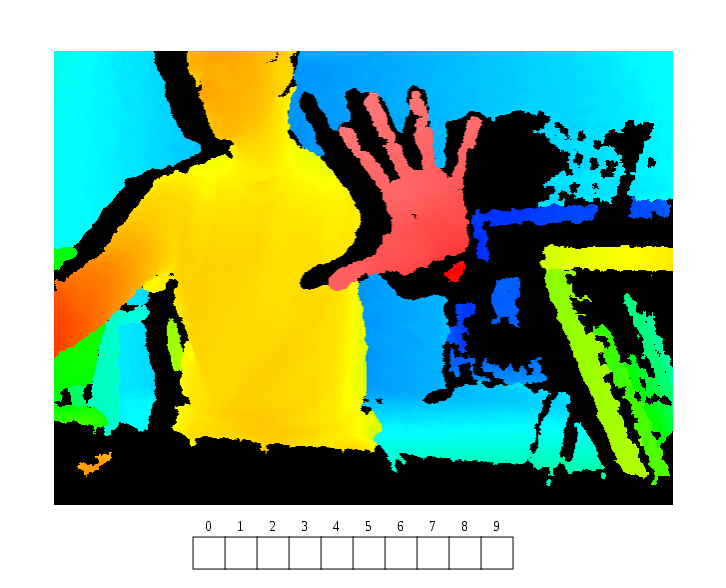
\includegraphics[width=0.6\linewidth]{kinect_array.png}
\end{figure}

\end{frame}
%%%%%%%%%%%%%%%%%%%
\begin{frame}

\begin{figure}

\includegraphics[width=0.6\linewidth]{openni.jpg}
\end{figure}

\end{frame}

%%%%%%%%%%%%%%%%

\begin{frame}

Class archivos
 
\begin{itemize}
\item int getCantLineas();
\item void guardarEnArreglo();
\item void setCantLineas();
\end{itemize}

\end{frame}

%%%%%%%%%%%%%%%%%%%%%%%%%%%%

\begin{frame}

Class conversion
 
\begin{itemize}
\item double convertir(string* pjoint1, string* pjoint2, int  n);
\item void llenarArregloAngulos();
\item double * getArregloAngulos();
\end{itemize}

\end{frame}
%%%%%%%%%%%%%%%%%%%%%%%%%%%%%%%


\begin{frame}

Class compara
 
\begin{itemize}
\item double * sacapromedios(double * arreglo);
\item int * arreglo\_promedio(double *arreglo\_prom1, double *arreglo\_prom2);
\item void comparar\_angulos(int * promedio);
\item void comparar\_velocidad(int pSizeMov1, int pSizeMov2);
\end{itemize}

\end{frame}

%----------------------------------------------------------------------------------------

\end{document} 
